\subsection{研究背景}
「優美さ」とは,図\ref{hogarth_curve}のような「美の線」を多く含むものであるとHogarthは説いた.
我々の研究室ではこの規範に則り,動作解析や動作生成を行ってきた.
これまでの研究では,解析に使用できる動作データは現在保有するcsvデータに限られていた.
最終的な優美評価はアンケートによる主観評価で,これもデータ量として少ないものであった.

近年,深層学習は大きな発展を見せている.
Recurrent Neural Network\cite{rnn}はConvolutional Neural Network\cite{cnn}にはない
「時間」という概念を持ち,機械翻訳の分野で大きな成果を出した.
一方で,小説などの大きな入力には対応できないという欠点もあった.
RNNに長期的記憶の概念を導入したLSTM\cite{lstm}やGRU\cite{gru}も開発されたが,
計算時間の増加が問題であった.

2017年に登場したTransformer\cite{transformer}は単純な行列計算のみで完結したネットワークで,
機械翻訳でこれまでのRNNを超える精度を出し,計算時間も大幅に削減したことで,
機械翻訳のデファクトスタンダードとなった.
2020年にはVision Transformer\cite{vit}が開発され,画像認識でCNNを超える精度を出した.
さらに翌年にはVideo Vision Transformer\cite{vivit}が開発され,動画解析でもRNNを超える精度を出した.

これまでViViTは物体検出などに用いられてきたが,上田研のテーマとする「優美さ」と言った
定量化しにくい対象に対しても応用できるのではないかと考えた.
これが成功すれば,先に挙げたデータの増加や評価の自動化など,研究をより円滑に進められる上に,
機械分類と人間の主観の差異も研究することができる.

\begin{figure}[b]
  \begin{center}
   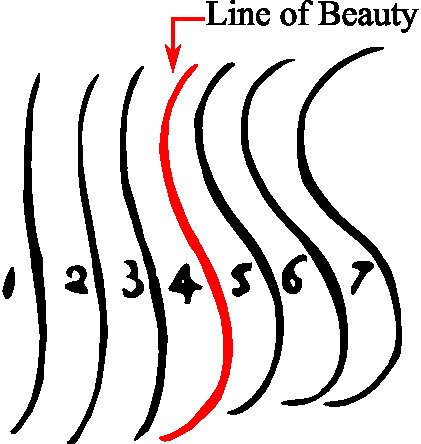
\includegraphics[width=50mm]{images/hogarth_curve.pdf}
  \end{center}
  \caption{Hogarth Curve}
  \label{hogarth_curve}
\end{figure}

\clearpage

\subsection{研究目的}

\subsection{研究概要}